% ==================================================
% CHAPTER 7: EVALUATION
% ==================================================

\chapter{Evaluation}
\label{ch:evaluation}

No public benchmark exists for hostel room swapping, so the engine is
evaluated on reproducible synthetic cohorts. Two studies were run: a
frozen 30-student cohort that checks the engine's guarantees and the
value of Murty's algorithm, and a benchmark over ten seeded 300-student
cohorts that chose the chain-length cap.

\section{Metrics}

\begin{itemize}
  \item \textbf{Cohort satisfaction}: the mean score over \emph{every}
  student in the cohort, before and after a round, not only over those
  who move. Averaging over movers alone would rank a two-person swap in
  which both reach 100\% above an eleven-person rotation that lifts the
  whole cohort.
  \item \textbf{Exact room}: students who get the exact room they named.
  \item \textbf{Worse off}: students whose score falls. This must be
  zero by construction; it is measured anyway, to confirm the filter
  works on real data and not only in unit tests.
  \item \textbf{Longest chain}: the largest number of students who must
  all approve before one chain executes.
  \item \textbf{Offered}: students who receive at least one executable
  chain.
  \item \textbf{Served}: students who can move at the same time, since
  offered chains compete for the same rooms.
\end{itemize}

\section{Frozen 30-Student Cohort}

The cohort has 30 students in one hostel, one per room, drawn once from
a seeded generator and frozen in \texttt{demo\_data.py}. Each student's
priorities follow a fallback ladder: a named room is worth more than its
floor, which is worth more than its direction. The cohort is run through
the service's own \texttt{/api/demo} endpoint, which uses the same
pipeline as a live round.

\subsection{Effect of Murty's Algorithm}

The best plan for the cohort was computed with $K = 1$ (Hungarian only),
$K = 50$ (the live default) and $K = 80$ (the prototype's setting),
choosing the assignment with the highest cohort satisfaction and, among
equals, the shortest longest chain.

\begin{table}[H]
\centering
\begin{tabular}{lccc}
\toprule
\textbf{Metric} & $K=1$ & $K=50$ & $K=80$ \\
\midrule
Cohort satisfaction, before $\to$ after & 11\% $\to$ 77\% & 11\% $\to$ 77\% & 11\% $\to$ 77\% \\
Students moved & 28 / 30 & 28 / 30 & 28 / 30 \\
Exact requested room & 20 / 30 & 20 / 30 & 20 / 30 \\
Worse off & 0 & 0 & 0 \\
Chains & 1 & 3 & 3 \\
Longest chain & 28 & 11 & 11 \\
Run time & 0.03\,s & 0.15\,s & 0.16\,s \\
\bottomrule
\end{tabular}
\caption{Best plan for the frozen 30-student cohort}
\label{tab:demo-k}
\end{table}

Satisfaction, the number of students moved and the number who get their
exact room are identical for all three values of $K$. Exploring
alternatives costs no match quality on this cohort. What changes is
\emph{executability}: with the Hungarian solution alone, all 28 movers
form a single chain, so one hold-out anywhere blocks everyone. With
Murty's alternatives the same outcome splits into three independent
chains, the longest of eleven. This is the concrete justification for
Murty's algorithm: a single solve is enough if quality is all that
matters, but an assignment that cannot realistically be approved is not
a useful answer. Nobody was worse off in any configuration.

The golden scenario tests show the same effect in miniature: in a small
hostel where no pair can swap but a three-way rotation works, $K = 1$
finds nothing executable and $K = 2$ finds the rotation.

\subsection{Options per Student}

Table~\ref{tab:demo-offers} shows the chains the live engine offers on
the same cohort ($K = 50$, up to three chains per student).

\begin{table}[H]
\centering
\begin{tabular}{lcc}
\toprule
\textbf{Metric} & \textbf{No cap} & \textbf{Cap 8} \\
\midrule
Distinct chains offered & 25 & 6 \\
Students with at least one offer & 28 / 30 & 17 / 30 \\
Longest offered chain & 26 & 7 \\
Run time & 0.06\,s & 0.05\,s \\
\bottomrule
\end{tabular}
\caption{Chains offered per student, frozen 30-student cohort}
\label{tab:demo-offers}
\end{table}

Without a cap almost everyone gets an offer, but some offers ask 26
students to agree. With the cap of eight, 17 students get an offer that
needs at most seven people to agree. On a cohort this small, a long
chain is most of the hostel; the cap's real effect shows only on larger
cohorts, which the next study measures.

\section{Chain-Cap Benchmark}
\label{sec:chain-cap}

\subsection{Set-up}

\begin{itemize}
  \item \textbf{Cohorts}: ten seeded synthetic cohorts of 300 students in
  one hostel (seeds 1--10, \texttt{hostelswap.synth.generator}). Mean
  satisfaction before any swap: 34.4\%.
  \item \textbf{Search}: Hungarian plus Murty with $K = 200$, run once
  per cohort and shared by all caps.
  \item \textbf{Caps}: 5, 8 and 10 students per chain.
  \item \textbf{Cost}: 51--68\,s of search per cohort; the whole study ran
  in 9.5 minutes, in memory.
\end{itemize}

\subsection{Results}

\begin{table}[H]
\centering
\begin{tabular}{cccccc}
\toprule
\textbf{Cap} & \textbf{Offered \%} & \textbf{Served \%} & \textbf{Satisfaction \%} & \textbf{Chains} & \textbf{Mean length} \\
\midrule
5  & $28.0 \pm 7.2$ & $23.5 \pm 5.6$ & $47.7 \pm 3.3$ & $28.0 \pm 7.2$  & $3.6 \pm 0.1$ \\
8  & $57.8 \pm 8.8$ & $42.7 \pm 6.2$ & $58.9 \pm 4.0$ & $53.0 \pm 12.0$ & $5.2 \pm 0.2$ \\
10 & $71.9 \pm 9.0$ & $46.5 \pm 7.0$ & $61.0 \pm 4.1$ & $68.1 \pm 14.2$ & $6.2 \pm 0.2$ \\
\bottomrule
\end{tabular}
\caption{Chain-cap benchmark: mean $\pm$ standard deviation over ten 300-student cohorts ($K = 200$)}
\label{tab:cap}
\end{table}

\begin{itemize}
  \item Raising the cap from 5 to 10 more than doubles the share of
  students who get any offer, from 28\% to 72\%.
  \item The three caps never overlap across cohorts: the worst cohort at
  cap 10 still beats the best cohort at cap 5 by 10 points. Within one
  cap, cohorts differ by up to 24 points, which is why ten runs were
  needed rather than one.
  \item \emph{Served} barely moves from cap 8 (42.7\%) to cap 10
  (46.5\%). Long chains compete for the same rooms, so the extra reach
  of cap 10 buys choice more than throughput.
\end{itemize}

\subsection{Why the Cohort Must Be Large}

Figure~\ref{fig:scale} shows the share of students offered a chain as
the cohort grows.

\begin{figure}[H]
\centering
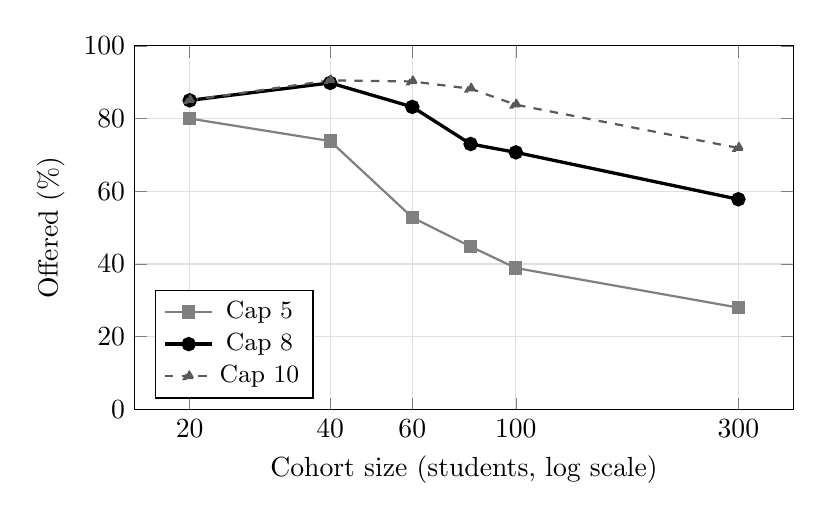
\begin{tikzpicture}
\begin{axis}[
  width=0.82\textwidth, height=6.2cm,
  xmode=log, log basis x=10,
  xlabel={Cohort size (students, log scale)},
  ylabel={Offered (\%)},
  xtick={20,40,60,100,300},
  xticklabels={20,40,60,100,300},
  ymin=0, ymax=100,
  legend pos=south west,
  legend style={font=\small},
  grid=major, grid style={gray!25},
  mark size=2pt,
]
\addplot[thick, mark=square*, gray] coordinates {(20,80.0) (40,73.8) (60,52.8) (80,44.8) (100,38.9) (300,28.0)};
\addplot[very thick, mark=*, black] coordinates {(20,85.0) (40,89.8) (60,83.2) (80,73.0) (100,70.7) (300,57.8)};
\addplot[thick, dashed, mark=triangle*, gray!70!black] coordinates {(20,85.0) (40,90.5) (60,90.2) (80,88.2) (100,83.8) (300,71.9)};
\legend{Cap 5, Cap 8, Cap 10}
\end{axis}
\end{tikzpicture}
\caption{Share of students offered a chain, by cohort size and cap}
\label{fig:scale}
\end{figure}

At 20 students a chain of ten is half the hostel, so the cap barely
binds and all three settings land within five points of each other. At
300 students the cap-5 and cap-10 lines are 44 points apart. A small
demonstration cohort would have hidden the effect entirely.

\subsection{Decision}

\textbf{Cap 8 is the operating point.} It reaches 58\% of the cohort and
raises satisfaction to 58.9\%. Cap 10 adds 14 points of reach for two
points of satisfaction, at the price of two more people per chain who
all have to agree, and it serves only four points more students at once.
The cap was then built into the engine (\texttt{max\_chain}) with eight as
the default, and a warden can change it per run.

One caveat: the benchmark used $K = 200$, while a live round uses
$K = 50$ to keep a run fast. On large cohorts the smaller search finds
fewer chains, so live figures will be below those in
Table~\ref{tab:cap}. The faster search in
Section~\ref{sec:performance} makes a larger live $K$ affordable.

\section{Performance}
\label{sec:performance}

\subsection{Complexity}

The Hungarian algorithm assigns one student per phase, and each phase
finds a shortest augmenting path while updating the dual potentials
over the $n \times n$ matrix in $O(n^2)$. With $n$ phases a solve is
$O(n^3)$. SciPy's \texttt{linear\_sum\_assignment} uses this
shortest-augmenting-path method (Jonker--Volgenant style). For a dense
matrix of arbitrary real costs no asymptotically faster exact method is
used in practice, so the gain has to come from how often, and on how
large a matrix, the solver is called.

That is decided by Murty's algorithm: $K$ results with up to $n$
subproblems each, every one an $O(n^3)$ solve, gives $O(Kn^4)$ in the
worst case. For $n = 300$ and $K = 200$ that is tens of thousands of
solves, which is why the benchmark needed about a minute per cohort.

\subsection{Optimisation}

Two inefficiencies were removed (Section~\ref{ch:implementation}):
fixed edges are now deleted from the matrix instead of being forced with
$\infty$, so subproblems shrink as Murty's search goes deeper, and
student and slot positions are looked up in $O(1)$ instead of $O(n)$.
Table~\ref{tab:speedup} compares the two versions on the same cohorts.

\begin{table}[H]
\centering
\begin{tabular}{rrrrrc}
\toprule
\textbf{Students} & \textbf{Before} & \textbf{After} & \textbf{Speed-up} & \textbf{Solves before / after} & \textbf{Same results} \\
\midrule
100 & 0.54\,s & 0.13\,s & 4.1$\times$ & 16\,457 / 9\,992 & yes \\
200 & 4.31\,s & 1.01\,s & 4.3$\times$ & 42\,988 / 23\,523 & yes \\
300 & 14.27\,s & 1.07\,s & 13.4$\times$ & 66\,681 / 24\,161 & yes \\
\bottomrule
\end{tabular}
\caption{Murty's search with $K = 50$, mean over five seeded cohorts per size (\commit{b8c78a7})}
\label{tab:speedup}
\end{table}

All fifteen cohorts returned exactly the same $K$ best costs before and
after, and a new test checks the first 20 assignments of a generated
pool against a brute-force search over all 720. The number of solves
also fell: many assignments differ by less than floating-point
rounding, so the order in which Murty's search breaks near-ties changes
with the solver, and with it the number of subproblems explored. For
the same reason individual run times vary; the table reports means.

\subsection{Run Times}

On the 30-student cohort a full run takes 0.15\,s at $K = 50$, and a
golden test asserts that a 100-student run finishes in under ten
seconds. A run happens once per round, behind the warden's ``lock and
run'' button, and its results are stored in
\texttt{round\_chain\_options}, so page loads never repeat it.

\subsection{Further Optimisation}

\begin{itemize}
  \item \textbf{Warm starts.} A Murty subproblem differs from its parent
  by one forbidden edge. Reusing the parent's dual potentials, only one
  augmenting path ($O(n^2)$) is needed instead of a full solve, which
  would bring the search to about $O(Kn^3)$. SciPy cannot be started
  from given potentials, so this needs our own Jonker--Volgenant
  implementation.
  \item \textbf{Parallel subproblems.} The $n$ children of one node are
  independent and can be solved in a process pool, for a constant-factor
  gain.
  \item \textbf{Pruning tested and rejected.} Forbidding, before the
  solve, every edge that would make a student worse off was tried on
  nine cohorts of 60--150 students. It gave no consistent gain in reach
  or speed, so it was not adopted.
\end{itemize}

\section{Threats to Validity}

\begin{itemize}
  \item All cohorts are synthetic. Real students may state preferences
  that are more alike (everyone wants the same floor), which would lower
  every figure here.
  \item The frozen cohort has one student per room, so shared rooms and
  roommate requests, though supported and unit-tested, are not part of
  these measurements.
  \item \emph{Offered} counts possibilities, not outcomes: the benchmark
  does not model whether students actually accept.
\end{itemize}
